\section{Tema 2. Equivalencia homotópica}

\subsection{Motivación: Homeomorfismo vs. Homotopía}

Sean $X, Y$ espacios topológicos. Decimos que $X$ e $Y$ son homeomorfos cuando $\exists f \colon X \to Y$ homeomorfismo ($f$ continua, biyectiva, $f^{-1}$ continua).

Equivalentemente: $X \cong Y \iff \exists f \colon X \to Y$ continua, $\exists g \colon Y \to X$ continua, tales que $f \circ g = 1_Y$ y $g \circ f = 1_X$.

\begin{nota}{Notación}{nota_homeomorfismo}
$X \cong Y$ significa que $X$ e $Y$ son homeomorfos. La aplicación identidad en $X$ se denota $1_X \colon X \to X$, $x \mapsto x$ (también se usa $id_X, i_X$).
\end{nota}

En este tema relajaremos las condiciones de la definición de homeomorfismo para llegar a la noción de espacios del mismo tipo de homotopía. Buscamos definir una especie de forma fundamental constante ante contracciones (como ilustra la reducción de un cilindro a una circunferencia o de un cono a un vértice).

\begin{center}
\begin{tikzpicture}[scale=0.8]
  % Cilindro a circunferencia
  \draw (0,2) ellipse (0.8 and 0.3);
  \draw (-0.8,0) -- (-0.8,2);
  \draw (0.8,0) -- (0.8,2);
  \draw (-0.8,0) arc (180:360:0.8 and 0.3);
  \draw[dashed] (0.8,0) arc (0:180:0.8 and 0.3);
  \draw[->] (1.5,1) -- (2.5,1);
  \draw (4,1) ellipse (0.8 and 0.3);
  \node at (0, 2.8) {$X$};
  \node at (4, 1.8) {$Y$};

  % Cono a punto
  \begin{scope}[yshift=-4cm]
      \draw (0,2) -- (-1,0) arc (180:360:1 and 0.3) -- cycle;
      \draw[dashed] (1,0) arc (0:180:1 and 0.3);
      \draw[->] (1.5,1) -- (2.5,1);
      \filldraw (4,1) circle (2pt);
      \node at (0, 2.5) {$\Delta$};
  \end{scope}
\end{tikzpicture}
\end{center}

\subsection{Homotopía entre aplicaciones}

\begin{definicion}{Homotopía entre aplicaciones}{def_homotopia}
Sea $f \colon X \to Y$ aplicación continua. \\
Sea $g \colon X \to Y$ aplicación continua.

Diremos que $f, g$ son homotópicas cuando $\exists F \colon X \times I = [0,1] \to Y$ continua tal que $F_0 = f, F_1 = g$.
\end{definicion}

\begin{nota}{Notación}{nota_homotopia}
Sea $t \in [0,1]$, definimos $F_t \colon X \to Y$ como $x \mapsto F(x,t)$.
\end{nota}

\begin{center}
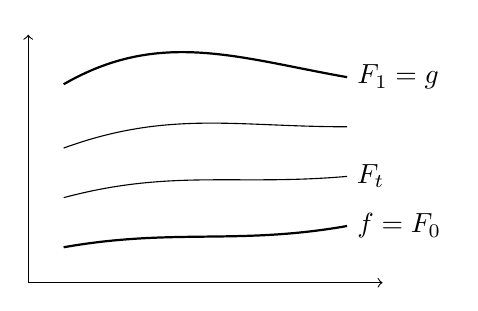
\begin{tikzpicture}[scale=0.9]
    \draw[->] (0,0) -- (0,3.5);
    \draw[->] (0,0) -- (5,0);
    
    \draw[thick] (0.5, 0.5) to[out=10, in=190] (4.5, 0.8) node[right] {$f = F_0$};
    \draw (0.5, 1.2) to[out=15, in=185] (4.5, 1.5) node[right] {$F_t$};
    \draw (0.5, 1.9) to[out=20, in=180] (4.5, 2.2);
    \draw[thick] (0.5, 2.8) to[out=30, in=170] (4.5, 2.9) node[right] {$F_1 = g$};
\end{tikzpicture}
\end{center}

$F$ captura una transformación parametrizada y continua entre $f$ y $g$.

\vspace{0.5cm}
\textbf{Ejemplos:} ¿$f$ y $g$ son homotópicas?

Recordemos que $S^n = \{x \in \mathbb{R}^{n+1} \mid |x| = 1\}$.

\begin{enumerate}
    \item $f \colon S^1 \to S^1, \quad z \mapsto z$ \\
    $g \colon S^1 \to S^1, \quad z \mapsto -z$
    
    $F \colon S^1 \times I \to S^1$ \\
    $(z, t) \mapsto z(\cos(\pi t) + i \sin(\pi t))$. 
    
    Como $F$ es continua y $F_0 = f, F_1 = g$, concluimos que $f$ y $g$ son homotópicas.
    
    \item $f \colon \mathbb{R}^2 \to \mathbb{R}^2, \quad (x,y) \mapsto (x,0)$ \\
    $g \colon \mathbb{R}^2 \to \mathbb{R}^2, \quad (x,y) \mapsto (0,y)$
    
    $F \colon \mathbb{R}^2 \times I \to \mathbb{R}^2$ \\
    $((x,y), t) \mapsto ((1-t)x, ty)$
    
    Por tanto $f$ y $g$ son homotópicas ($f \simeq g$).
\end{enumerate}

\subsubsection{Estructura en $C(X,Y)$}

Llamamos $C(X,Y) = \{f \colon X \to Y \mid f \text{ continua}\}$. Vimos que $\simeq$ es R.B.E en $C(X,Y)$. Luego podemos hablar del conjunto cociente $C(X,Y)/\simeq$, que se suele denotar por $[X,Y]$.

\begin{teorema}{Relación de equivalencia en $C(X,Y)$}{teo_rel_eq}
La homotopía $\simeq$ es una Relación de Equivalencia (R.B.E.) en $C(X,Y)$.
\end{teorema}

\begin{proof}
\begin{enumerate}
    \item \textbf{Reflexiva:} $\forall f \in C(X,Y) \colon f \simeq f$. Basta definir $F \colon X \times I \to Y$ continua mediante $(x,t) \mapsto f(x)$. Evaluando, $F_0 = f$ y $F_1 = f$.
    \item \textbf{Simétrica:} $\forall f,g \in C(X,Y) \colon f \simeq g \implies g \simeq f$.
    Dado que $f \simeq g$, $\exists F \colon X \times I \to Y$ continua tal que $F_0 = f, F_1 = g$.
    Buscamos una $G \colon X \times I \to Y$ continua con $G_0 = g, G_1 = f$.
    Definimos $G(x,t) = F(x, 1-t)$. Es continua por ser composición de funciones continuas y cumple $G_0 = F_1 = g$ y $G_1 = F_0 = f$.
    \item \textbf{Transitiva:} $\forall f,g,h \in C(X,Y) \colon f \simeq g, g \simeq h \implies f \simeq h$.
    Suponemos que $f \simeq^{(1)} g$ y $g \simeq^{(2)} h$. Esto implica que existen $F^{(1)} \colon X \times [0,1] \to Y$ y $F^{(2)} \colon X \times [0,1] \to Y$.
    Necesitamos construir $F \colon X \times I \to Y$ continua con $F_0 = f$ y $F_1 = h$. Definimos:
    \[ F(x,t) = \begin{cases} F^{(1)}(x, 2t) & \forall t \in \left[0, \frac{1}{2}\right] \\ F^{(2)}(x, 2t-1) & \forall t \in \left[\frac{1}{2}, 1\right] \end{cases} \]
    Como $\left(X \times \left[0,\frac{1}{2}\right]\right)$ y $\left(X \times \left[\frac{1}{2}, 1\right]\right)$ son cerrados con restricción continua en la intersección, entonces $F$ es continua. Comprobamos la frontera:
    $F\left(x, \frac{1}{2}\right) = F^{(1)}(x,1) = g(x)$ y $F\left(x, \frac{1}{2}\right) = F^{(2)}(x,0) = g(x)$. Tenemos $F$ bien definida.
    $F_0(x) = F(x,0) = F^{(1)}(x,0) = f(x), \forall x \in X$.
    $F_1(x) = F(x,1) = F^{(2)}(x,1) = h(x), \forall x \in X$.
    Como consecuencia de todo lo anterior, $f \simeq h$.
\end{enumerate}
Por tanto, podremos hablar del espacio cociente $C(X,Y)/\simeq$.
\end{proof}

\begin{teorema}{Composición de homotopías}{teo_comp_homo}
Sean $X \xrightarrow{f_1, f_2} Y \xrightarrow{g_1, g_2} Z$. Si suponemos que $f_1 \simeq f_2$ y $g_1 \simeq g_2$, entonces $g_1 \circ f_1 \simeq g_2 \circ f_2$.
\end{teorema}

\begin{proof}
Tenemos $F \colon X \times I \to Y$ continua con $F_0=f_1, F_1=f_2$.
Tenemos $G \colon Y \times I \to Z$ continua con $G_0=g_1, G_1=g_2$.
Definimos la aplicación $H \colon X \times I \to Z$, $(x,t) \mapsto G(F(x,t), t)$. Evaluamos en los extremos:
\[ H_0(x) = H(x,0) = G(F(x,0), 0) = G(f_1(x), 0) = G_0(f_1(x)) = g_1(f_1(x)), \forall x \in X. \]
\[ H_1(x) = H(x,1) = G(F(x,1), 1) = G(f_2(x), 1) = G_1(f_2(x)) = g_2(f_2(x)), \forall x \in X. \]
Como $H$ es continua, queda probado que $g_1 \circ f_1 \simeq g_2 \circ f_2$.
\end{proof}


\subsection{Equivalencia homotópica entre espacios}

\begin{definicion}{Equivalencia homotópica}{def_eq_homotopica}
Sean $X, Y$ espacios topológicos. Diremos que $X$ e $Y$ son del mismo tipo de homotopía ($X \simeq Y$) cuando $\exists f \colon X \to Y$ continua y $\exists g \colon Y \to X$ continua tales que $f \circ g \simeq 1_Y$ y $g \circ f \simeq 1_X$. 

En este caso también diremos que $f$ es una \textbf{equivalencia homotópica} y $g$ la \textbf{inversa homotópica} de $f$ (no necesariamente $f$ biyectiva).
\end{definicion}

\begin{observacion}{Relación con el homeomorfismo}{obs_iso}
$X \cong Y \implies X \simeq Y$ (y $g$ es inversa de $f$).
Tomando $f \colon X \to Y, g \colon Y \to X$ biyecciones donde $g \circ f = 1_X$ y $f \circ g = 1_Y$, se sigue que son trivialmente homotópicas a las identidades ($g \circ f \simeq 1_X$ y $f \circ g \simeq 1_Y$).

Sin embargo, $f \colon X \to Y$ continua y biyectiva $\not\implies f^{-1}$ continua (y no necesariamente $f$ es equivalencia homotópica si falla el homeomorfismo). Como contraejemplo:
$f \colon [0, 1) \to S^1, \quad t \mapsto (\cos(2\pi t), \sin(2\pi t))$.
\end{observacion}

\begin{nota}{Invarianza por eliminación de puntos}{nota_agujeros}
Como consecuencia de las propiedades topológicas: si $X \cong Y$, dado $P \in X$, entonces $X \setminus \{P\} \cong Y \setminus \{f(P)\}$. Para el caso homotópico, la pregunta análoga es si $\forall P \in X, \exists Q \in Y$ tal que $X \setminus \{P\} \simeq Y \setminus \{Q\}$.
\end{nota}

\textbf{Ejemplos:}
\begin{enumerate}
    \item Sea $X = D(0,1) = \{(x,y) \in \mathbb{R}^2 \mid ||(x,y)|| < 1\}$ y $Y = \{(0,0)\}$.
    Definimos $f \colon X \to Y$, $f = \text{cte}$, es decir, $f(x,y) = (0,0), \forall (x,y) \in X$.
    Definimos $g \colon Y \to X$, $g(0,0) = (0,0)$.
    
    Tenemos que $f \circ g(0,0) = (0,0) \implies f \circ g = 1_Y \implies f \circ g \simeq 1_Y$.
    Y también $g \circ f(x,y) = g(0,0) = (0,0), \forall (x,y) \in X \implies g \circ f = c_{(0,0)}$.
    
    Sea $F \colon X \times I \to X$ continua dada por $F((x,y), t) = t \cdot (x,y)$. Se tiene $F_0 = c_{(0,0)}$ y $F_1 = 1_X$. Por tanto, $g \circ f \simeq 1_X$, y concluimos que $X \simeq Y$.
    
    \item Sean $X = [-1,1]$ y $Y = [-1,1] \times \{0\} \cup \{0\} \times [-1,1]$. 
    Evaluando el número de componentes conexas al quitar un punto: $\mathcal{O}(X) = \{1, 2\}$ y $\mathcal{O}(Y) = \{1, 2, 4\}$. Como $\mathcal{O}(X) \neq \mathcal{O}(Y) \implies X \not\cong Y$. Sin embargo, se puede demostrar que $X \simeq Y$.
    
    \item Sean $X = S^1 \times [-1,1]$ (cilindro) y $Y = S^1$.
    $f \colon X \to Y, (x,y,z) \mapsto (x,y)$.
    $g \colon Y \to X, (x,y) \mapsto (x,y,0)$.
    
    $f \circ g(x,y) = f(x,y,0) = (x,y) = id_Y, \forall (x,y) \in Y$.
    $g \circ f(x,y,z) = g(x,y) = (x,y,0)$. 
    Construimos $F \colon X \times I \to X$ dada por $F((x,y,z), t) = (x,y, t \cdot z)$. Se verifica que $F_0 = g \circ f$ y $F_1 = 1_X \implies X \simeq Y$.
\end{enumerate}


\subsection{Espacios Contractiles, Convexos y Estrellados}

\begin{definicion}{Espacio topológico contractil}{def_contractil}
Un espacio topológico $X \neq \emptyset$ es contractil si $\exists x_0 \in X \mid 1_X \simeq c_{x_0}$ (donde $c_{x_0}$ es la aplicación constante $x \mapsto x_0$).
\end{definicion}

\begin{teorema}{Caracterización de espacios contractiles}{teo_contractil}
Son equivalentes las siguientes afirmaciones para un e.t. $X \neq \emptyset$:
\begin{enumerate}
    \item[a)] $X$ es contractil.
    \item[b)] $id_X \simeq c_x, \forall x \in X$.
    \item[c)] $\forall f,g \colon T \to X$ continuas $\implies f \simeq g$ (para cualquier e.t. $T$).
    \item[d)] $X$ es del mismo tipo de homotopía que un punto.
\end{enumerate}
\end{teorema}

\begin{definicion}{Conjunto convexo}{def_convexo}
Sea $X \subseteq \mathbb{R}^n$. Diremos que $X$ es convexo cuando todo segmento que une dos puntos cualesquiera de $X$ está contenido en $X$. Equivalentemente:
\[ \exists x_0 \in X \mid \forall x \in X, \forall t \in [0,1]: \quad tx + (1-t)y \in X \]
\end{definicion}

\begin{teorema}{Contracción de conjuntos convexos}{teo_convexo_contractil}
Todo subconjunto convexo de $\mathbb{R}^n$ es contractil (del mismo tipo de homotopía que un punto).
\end{teorema}

\begin{proof}
Sea $x_0 \in X$. Tomamos un punto cualquiera de $X$ y definimos:
\[ f \colon X \to \{x_0\} \hookrightarrow X, \quad x \mapsto x_0 \]
\[ g \colon \{x_0\} \to X, \quad x_0 \mapsto x_0 \]
Claramente $f \circ g = 1_{\{x_0\}}$. Veamos que $g \circ f = c_{x_0} \simeq 1_X$. Definimos la homotopía $F \colon X \times I \to X$ como:
\[ F(x,t) = tx + (1-t)x_0 \]
Evaluando en los extremos, $F_0(x) = x_0 = c_{x_0}$ y $F_1(x) = x = 1_X$. Luego $g \circ f \simeq 1_X$.
\end{proof}

\begin{definicion}{Conjunto estrellado}{def_estrellado}
Sea $X \subseteq \mathbb{R}^n$. Diremos $X$ estrellado cuando $\exists x_0 \in X$ tal que todo segmento que une $x_0$ con algún punto de $X$, esté contenido en $X$. Equivalentemente:
\[ X \text{ estrellado} \iff \exists x_0 \in X \mid \forall x \in X, \forall t \in [0,1]: \quad tx + (1-t)x_0 \in X \]
\end{definicion}

\begin{observacion}{}{obs_convexo_estrellado}
Todo conjunto convexo es estrellado (Convexo $\implies$ estrellado).
\end{observacion}

\begin{teorema}{Contracción de conjuntos estrellados}{teo_estrellado_contractil}
Sea $X \subseteq \mathbb{R}^n$. Si $X$ es estrellado $\implies X$ es contractil.
\end{teorema}
\begin{proof}
Análogo a la demostración del teorema de espacios convexos, utilizando el punto central $x_0$ que define el conjunto estrellado para construir la homotopía de contracción.
\end{proof}


\subsection{Homotopía relativa y Grupo Fundamental}

Sea $X$ e.t., $x_0, x_1 \in X$. Al conjunto $C_{x_0, x_1}(X) = \{ \alpha \colon [0,1] \to X \text{ cont } \mid \alpha(0) = x_0, \alpha(1) = x_1 \}$ se le denomina conjunto de arcos o caminos. 

Saber que dos arcos cualesquiera son homotópicos no es suficiente para "cazar" agujeros topológicos. Por ello, requerimos fijar subconjuntos durante la deformación.

\begin{definicion}{Homotopía relativa}{def_homotopia_relativa}
Sea $A \subseteq X$. Sean $f, g \colon X \to Y$ continuas. Diremos que $f, g$ son homotópicas respecto a $A$ (denotado $f \simeq_A g$) cuando $\exists F \colon X \times I \to Y$ continua tal que:
\begin{enumerate}
    \item $F_0 = f$
    \item $F_1 = g$
    \item $\forall a \in A, \forall t \in I \colon F(a,t)$ es constante (no depende de $t$). En particular, $F(a,t) = f(a) = g(a) \ \forall t \in I$.
\end{enumerate}
\end{definicion}

Para caminos con extremos fijos, $\alpha \simeq_{\{0,1\}} \beta \iff \exists F \colon I \times I \to X$ continua tal que:
1. $F_0 = \alpha$ \\
2. $F_1 = \beta$ \\
3. $F(0,t) = \alpha(0) = \beta(0)$, y $F(1,t) = \alpha(1) = \beta(1) \quad \forall t \in I$.

Si $x_0 = x_1$, notaremos $C_{x_0}(X)$ al conjunto de \textbf{lazos} con base en $x_0$.

\begin{teorema}{Relación de equivalencia relativa}{teo_rbe_relativa}
La relación $\simeq_A$ es una R.B.E. en $C(X,Y)$. 
\end{teorema}

\begin{definicion}{Grupo fundamental}{def_grupo_fundamental}
Sea $X$ e.t., sea $x_0 \in X$. Definimos el grupo fundamental de $X$ en $x_0$, denotado como $\pi_1(X, x_0)$, al conjunto cociente de lazos bajo homotopía relativa a los extremos:
\[ \pi_1(X, x_0) \equiv C_{x_0}(X) / \simeq_{\{0,1\}} \]
A la clase de equivalencia de un lazo $\alpha$ la denotamos como $[\alpha]$.
\end{definicion}

Para dotar a $\pi_1(X, x_0)$ de estructura de grupo, introducimos operaciones en caminos:
Sean $x_0, x_1, x_2 \in X$ y caminos $\alpha \colon I \to X$ (de $x_0$ a $x_1$) y $\beta \colon I \to X$ (de $x_1$ a $x_2$).
Definimos la \textbf{concatenación} $\gamma = \alpha * \beta \colon I \to X$ dada por:
\[ \gamma(t) = \begin{cases} \alpha(2t), & \forall t \in [0, 1/2] \\ \beta(2t-1), & \forall t \in [1/2, 1] \end{cases} \]
Definimos el \textbf{camino inverso} $\alpha^{-1} \colon I \to X$ como $\alpha^{-1}(t) = \alpha(1-t)$, el cual va de $x_1$ a $x_0$.

\begin{teorema}{Conexión por caminos}{teo_contractil_arcoconexo}
Sea $X$ contractil. Entonces $X$ es arco-conexo.
\end{teorema}
\begin{proof}
Sean $x, y \in X$. Por ser contractil, $\exists x_0 \in X \mid 1_X \simeq c_{x_0}$. Es decir, $\exists F \colon X \times I \to X$ continua con $F_0 = 1_X, F_1 = c_{x_0}$.
Definimos el camino $\alpha \colon I \to X$ dado por $t \mapsto F(x,t)$, que une $\alpha(0)=x$ con $\alpha(1)=x_0$.
Definimos el camino $\beta \colon I \to X$ dado por $t \mapsto F(y,t)$, que une $\beta(0)=y$ con $\beta(1)=x_0$.
El camino concatenado $\delta = \alpha * \beta^{-1}$ une los puntos $x$ e $y$ de forma continua.
\end{proof}

\begin{nota}{Asociatividad de caminos}{nota_asociatividad}
Es importante notar que $\alpha * (\beta * \gamma) \neq (\alpha * \beta) * \gamma$ a nivel de aplicaciones, ya que las parametrizaciones difieren en los intervalos temporales. Sin embargo, sí son equivalentes bajo homotopía relativa a los extremos. 
Definimos entonces el producto de clases como:
\[ [\alpha] \cdot [\beta] = [\alpha * \beta] \]
\end{nota}

\begin{teorema}{de Poincaré}{poincare}
Sea $X$ un espacio topológico y sea $x_0 \in X$. Entonces 
\[
(\pi_1(X, x_0), \cdot)
\]
es un grupo.
\end{teorema}

\begin{proof}
Dividimos la demostración en la comprobación de la buena definición de la operación y el cumplimiento de los axiomas de grupo:

\begin{enumerate}
    \item \textbf{La operación está bien definida.}
    
    Sean $\alpha, \alpha', \beta, \beta' \in \mathcal{C}_{x_0}(X)$. Se debe probar que:
    \[
    \left.
    \begin{aligned}
    \alpha &\simeq_{\{0,1\}} \alpha' \\
    \beta &\simeq_{\{0,1\}} \beta'
    \end{aligned}
    \right\} \implies \alpha * \beta \simeq_{\{0,1\}} \alpha' * \beta'
    \]
    Por hipótesis, existen homotopías relativas:
    \begin{itemize}
        \item $H^{(1)} : I \times I \to X$ continua con:
        \[
        H_0^{(1)} = \alpha, \quad H_1^{(1)} = \alpha', \quad H^{(1)}(0, t) = \alpha(0) = \alpha'(0) = x_0, \quad H^{(1)}(1, t) = \alpha(1) = \alpha'(1) = x_0 \quad (\forall t \in I)
        \]
        \item $H^{(2)} : I \times I \to X$ continua con:
        \[
        H_0^{(2)} = \beta, \quad H_1^{(2)} = \beta', \quad H^{(2)}(0, t) = x_0, \quad H^{(2)}(1, t) = x_0 \quad (\forall t \in I)
        \]
    \end{itemize}

    Se define la aplicación $H : I \times I \to X$ dada a trozos por:
    \[
    H(s, t) = 
    \begin{cases}
    H^{(1)}(2s, t) & \text{si } s \in [0, 1/2], \\
    H^{(2)}(2s - 1, t) & \text{si } s \in [1/2, 1].
    \end{cases}
    \]

    \begin{itemize}
        \item \emph{Coincidencia en la frontera común ($s = 1/2$):}
        \[
        H(1/2, t) = 
        \begin{cases}
        H^{(1)}\left(2 \cdot \frac{1}{2}, t\right) = H^{(1)}(1, t) = x_0, \\
        H^{(2)}\left(2 \cdot \frac{1}{2} - 1, t\right) = H^{(2)}(0, t) = x_0.
        \end{cases}
        \]
        Por tanto, $H$ está bien definida.

        \item \emph{Continuidad de $H$:}
        Escribimos $I \times I = B_1 \cup B_2$, donde:
        \[
        B_1 = [0, 1/2] \times I, \qquad B_2 = [1/2, 1] \times I
        \]
        Ambos subconjuntos son cerrados en $I \times I$. Como $H|_{B_1}$ y $H|_{B_2}$ son continuas y coinciden en $B_1 \cap B_2$, por el lema de pegamiento (continuidad a trozos), $H$ es continua.

        \item \emph{Instantes $t = 0$ y $t = 1$:}
        \[
        H_0(s) = H(s, 0) = 
        \begin{cases}
        H^{(1)}(2s, 0) = \alpha(2s) & \text{si } s \in [0, 1/2], \\
        H^{(2)}(2s - 1, 0) = \beta(2s - 1) & \text{si } s \in [1/2, 1],
        \end{cases}
        \implies H_0 = \alpha * \beta
        \]
        \[
        H_1(s) = H(s, 1) = 
        \begin{cases}
        H^{(1)}(2s, 1) = \alpha'(2s) & \text{si } s \in [0, 1/2], \\
        H^{(2)}(2s - 1, 1) = \beta'(2s - 1) & \text{si } s \in [1/2, 1],
        \end{cases}
        \implies H_1 = \alpha' * \beta'
        \]

        \item \emph{Fijación de los extremos ($s = 0$ y $s = 1$):}
        \[
        \begin{aligned}
        H(0, t) &= H^{(1)}(0, t) = x_0, \\
        H(1, t) &= H^{(2)}(1, t) = x_0.
        \end{aligned}
        \]
        No dependen de $t$. En consecuencia, $H : \alpha * \beta \simeq_{\{0,1\}} \alpha' * \beta'$.
    \end{itemize}

    \item \textbf{Propiedad asociativa.}
    
    Se debe probar que:
    \[
    [\alpha] \cdot ([\beta] \cdot [\gamma]) = ([\alpha] \cdot [\beta]) \cdot [\gamma], \quad \forall \alpha, \beta, \gamma \in \mathcal{C}_{x_0}(X)
    \]
    lo cual equivale a demostrar que $(\alpha * \beta) * \gamma \simeq_{\{0,1\}} \alpha * (\beta * \gamma)$.
    
    Explícitamente, las parametrizaciones son:
    \[
    ((\alpha * \beta) * \gamma)(s) = 
    \begin{cases}
    \alpha(4s) & \text{si } s \in [0, 1/4], \\
    \beta(4s - 1) & \text{si } s \in [1/4, 1/2], \\
    \gamma(2s - 1) & \text{si } s \in [1/2, 1];
    \end{cases}
    \]
    \[
    (\alpha * (\beta * \gamma))(s) = 
    \begin{cases}
    \alpha(2s) & \text{si } s \in [0, 1/2], \\
    \beta(4s - 2) & \text{si } s \in [1/2, 3/4], \\
    \gamma(4s - 3) & \text{si } s \in [3/4, 1].
    \end{cases}
    \]
    
    Se define la homotopía $H : I \times I \to X$ mediante reparametrizaciones afines a trozos sobre los intervalos que varían linealmente con $t$:
    \[
    H(s, t) = 
    \begin{cases}
    \alpha\left( \dfrac{4}{t + 1} s \right) & \text{si } s \in \left[ 0, \dfrac{t+1}{4} \right], \\[2ex]
    \beta(4s - t - 1) & \text{si } s \in \left[ \dfrac{t+1}{4}, \dfrac{t+2}{4} \right], \\[2ex]
    \gamma\left( \dfrac{4s - 2 - t}{2 - t} \right) & \text{si } s \in \left[ \dfrac{t+2}{4}, 1 \right].
    \end{cases}
    \]
    
    \begin{itemize}
        \item \emph{Buena definición en las fronteras:}
        \begin{itemize}
            \item En $s = \frac{t+1}{4}$:
            \[
            \alpha\left( \frac{4}{t+1} \cdot \frac{t+1}{4} \right) = \alpha(1) = x_0, \qquad \beta\left( 4 \cdot \frac{t+1}{4} - t - 1 \right) = \beta(0) = x_0.
            \]
            \item En $s = \frac{t+2}{4}$:
            \[
            \beta\left( 4 \cdot \frac{t+2}{4} - t - 1 \right) = \beta(1) = x_0, \qquad \gamma\left( \frac{4\frac{t+2}{4} - 2 - t}{2 - t} \right) = \gamma(0) = x_0.
            \]
        \end{itemize}
        \item \emph{Continuidad:} Por el lema de pegamiento en los subconjuntos cerrados determinados por las rectas $s = \frac{t+1}{4}$ y $s = \frac{t+2}{4}$, $H$ es continua.
        \item \emph{Evaluación en los extremos temporales:}
        \[
        H(s, 0) = ((\alpha * \beta) * \gamma)(s), \qquad H(s, 1) = (\alpha * (\beta * \gamma))(s).
        \]
        \item \emph{Extremos espaciales:}
        \[
        H(0, t) = \alpha(0) = x_0, \qquad H(1, t) = \gamma(1) = x_0 \quad (\forall t \in I).
        \]
    \end{itemize}
    Por tanto, $H$ es una homotopía relativa y la operación es asociativa.

    \item \textbf{Existencia de elemento neutro.}
    
    Sea $c_{x_0} : I \to X$ el lazo constante $c_{x_0}(s) = x_0$ para todo $s \in I$. Se debe probar que:
    \[
    [c_{x_0}] \cdot [\alpha] = [\alpha] \iff c_{x_0} * \alpha \simeq_{\{0,1\}} \alpha.
    \]
    El producto con el neutro es:
    \[
    (c_{x_0} * \alpha)(s) = 
    \begin{cases}
    c_{x_0}(2s) = x_0 & \text{si } s \in [0, 1/2], \\
    \alpha(2s - 1) & \text{si } s \in [1/2, 1].
    \end{cases}
    \]
    Se construye la homotopía $F : I \times I \to X$:
    \[
    F(s, t) = 
    \begin{cases}
    x_0 & \text{si } s \in \left[0, \dfrac{1-t}{2}\right], \\[2ex]
    \alpha\left( \dfrac{2s + t - 1}{t + 1} \right) & \text{si } s \in \left[\dfrac{1-t}{2}, 1\right].
    \end{cases}
    \]
    \begin{itemize}
        \item En $s = \frac{1-t}{2}$, $\alpha\left( \frac{2\frac{1-t}{2} + t - 1}{t+1} \right) = \alpha(0) = x_0$, coincidiendo con el valor constante.
        \item $F(s, 0) = (c_{x_0} * \alpha)(s)$ y $F(s, 1) = \alpha(s)$.
        \item $F(0, t) = x_0$ y $F(1, t) = \alpha(1) = x_0$ para todo $t \in I$.
    \end{itemize}
    Análogamente se comprueba para $[\alpha] \cdot [c_{x_0}] = [\alpha]$.

    \item \textbf{Existencia de elemento simétrico (inverso).}
    
    Para cada lazo $\alpha \in \mathcal{C}_{x_0}(X)$, se define el lazo inverso $\alpha^{-1} : I \to X$ como:
    \[
    \alpha^{-1}(s) = \alpha(1 - s).
    \]
    
    \begin{itemize}
        \item \emph{Buena definición de la clase inversa:} Si $\alpha \simeq_{\{0,1\}} \gamma$ mediante una homotopía $F(s, t)$, entonces $G(s, t) = F(1 - s, t)$ proporciona una homotopía relativa entre $\alpha^{-1}$ y $\gamma^{-1}$, por lo que $[\alpha]^{-1} = [\alpha^{-1}]$ está bien definido.
        \item \emph{Simétrico respecto al producto:} Falta probar que $[\alpha^{-1}] \cdot [\alpha] = [c_{x_0}]$, es decir, $\alpha^{-1} * \alpha \simeq_{\{0,1\}} c_{x_0}$.
    \end{itemize}
    La homotopía explícita $F : I \times I \to X$ viene dada por:
    \[
    F(s, t) = 
    \begin{cases}
    \alpha^{-1}(2s(1 - t)) = \alpha(1 - 2s(1 - t)) & \text{si } s \in [0, 1/2], \\[1ex]
    \alpha(2s(1 - t) + 2t - 1) & \text{si } s \in [1/2, 1].
    \end{cases}
    \]
    \begin{itemize}
        \item En $s = 1/2$:
        \[
        \alpha(1 - 2(1/2)(1 - t)) = \alpha(t), \qquad \alpha(2(1/2)(1 - t) + 2t - 1) = \alpha(t).
        \]
        \item Para $t = 0$: $F(s, 0) = (\alpha^{-1} * \alpha)(s)$.
        \item Para $t = 1$: $F(s, 1) = \alpha(1) = x_0 = c_{x_0}(s)$.
        \item En los extremos: $F(0, t) = \alpha(1) = x_0$ y $F(1, t) = \alpha(1) = x_0$ para todo $t \in I$.
    \end{itemize}
    El mismo procedimiento demuestra que $\alpha * \alpha^{-1} \simeq_{\{0,1\}} c_{x_0}$.
\end{enumerate}
Por tanto, $(\pi_1(X, x_0), \cdot)$ es un grupo.
\end{proof}
